\documentclass{article} % For LaTeX2e
\usepackage{nips12submit_e,times}
\usepackage{hyperref}
\usepackage[margin=1.5in]{geometry}
\usepackage{graphicx}

%\documentstyle[nips12submit_09,times,art10]{article} % For LaTeX 2.09


 \title{Digit Recognition: Nearest Neighbors vs. Perceptron}


\author{
Harnoor Singh \\
Department of Computer Science \& Engineering\\
University of Washington \\
\texttt{hsingh@cs.washington.edu} \\
\And
Brian Walker \\
Department of Computer Science \& Engineering \\
University of Washington \\
\texttt{bdwalker@cs.washington.edu} \\
}

% The \author macro works with any number of authors. There are two commands
% used to separate the names and addresses of multiple authors: \And and \AND.
%
% Using \And between authors leaves it to \LaTeX{} to determine where to break
% the lines. Using \AND forces a linebreak at that point. So, if \LaTeX{}
% puts 3 of 4 authors names on the first line, and the last on the second
% line, try using \AND instead of \And before the third author name.

\newcommand{\fix}{\marginpar{FIX}}
\newcommand{\new}{\marginpar{NEW}}

\nipsfinalcopy % Uncomment for camera-ready version

\begin{document}
\maketitle

\begin{abstract}

Optical Character Recognition (OCR) is a complex computer science problem which
has several effective machine learning solutions. We implemented the K Nearest
Neighbors (KNN) and Kernelized Perceptron algorithms and compared the
effectiveness of both methods in classifying a testing data set of 28,000
images. Each image is formatted as an array of 768 pixel values, with each value
indicating how dark each pixel was in the image. Both of our algorithms were
trained on a training data set of 42,000 images. We used cross validation to
tune the K value in KNN and to choose a kernel function and dimension value for
Perceptron. Despite its relative simplicity, we found that KNN was more
effective than Perceptron in classifying the digits. The nearest neighbors
algorithm correctly classified 96.857\% of the testing samples on a weighted
neighbors algorithm which looked at 4 neighbors. Our best Perceptron
implementation correctly classified 95.67\% of the testing samples using an
exponential kernel with a $\sigma = 5$. Despite its higher accuracy, the runtime
of KNN was 8x slower than that of the Perceptron.

\end{abstract}

\section{The Problem}

\subsection{Image Data}
Optical Character Recognition (OCR) is a computational problem where a machine
attempts to classify an image of text. We tackled a subset of this problem,
attempting to classify the digits 0-9 from data provided by the Kaggle Digit
Recognition
competition\footnote{\url{http://www.kaggle.com/c/digit-recognizer}}.

The Kaggle data provides two groups of data, 42,000 training samples with labels
and 28,000 unlabeled testing samples. Each training sample contains a 48 pixel
by 48 pixel image containing a handwritten number. The image is represented as
an array of 768 pixel values which represent how dark each pixel of the image
is. Table 1 is an example of a training sample.

\begin{table}[ht]
\textbf{\caption{Subset of Kaggle Data}} % title
\centering 
\begin{tabular}{c | c c c }
Label & Pixel 77 & Pixel 78 & Pixel 79 \\
\hline
8 & 0 & 0 & 0 \\
6 & 89 & 208 & 135 \\ [1ex]
\end{tabular}
\label{table:Data}
\end{table}

\section{K Nearest Neighbors (KNN)}

\subsection{Overview}

K Nearest Neighbors is a relatively simple algorithm which often gets surprisingly
good results given its simplicity. Given a testing sample $X$, the algorithm
looks through all the training samples it has previously seen and finds the
\textit{K} most similar samples. The algorithm then implements some form of
voting mechanism among the \textit{K} samples to classify the testing sample as
a digit 0-9. The voting mechanism can either be as straightforward as selecting the
majority label, to something more complicated which involves weighting the
samples based on some distance metric. 

\subsection{Implementation Details}

The first step in implementing KNN is to find the \textit{K} nearest
neighbors. This is accomplished by taking the euclidean distance between the
testing sample we are classifying and every training sample in our training data
set. 

\begin{center}
$Euclidean(TestX, TrainX) = \sum\limits_{i \in TrainX} {(TestX - TrainX_i)^2}$
\end{center}

Because the image data is defined as an array of 768 pixels, $TestX - TrainX_i$
is actually doing a 768 dimension comparison between data points.

Once we identified the \textit{K} nearest neighbors to our testing sample, we
had to use this information to classify the testing point. We considered two
approaches when deciding how to perform this classification.

\subsubsection{Unweighted KNN}

The first method we implemented to classify our testing sample was a simple
majority voting algorithm which selects the majority label from the \textit{K}
closest neighbors. For example, if we ran the nearest neighbors algorithm with
$K = 5$ and 3 of the neighbors had a label of 6, we would classify our testing
sample as a 6.

\subsubsection{Weighted KNN}

Given the \textit{K} nearest neighbors, the weighted version of the algorithm
multiplies each label by a weight which indicates how close it is to our testing
sample. These weights help to emphasize points that are closer to our testing
sample while reducing the impact further away training points have on
classifying our testing sample. 

\subsection{Cross Validation}

Our implementation of KNN has a number of parameters which require
tuning. In particular, we need to decide whether or not to use the weighted
version of our KNN algorithm and how many neighbors to consider when
implementing our algorithm.

To do this, we implemented K folds cross validation using 5,000 training
samples. The reduced training set allowed us to run our algorithm using various
configurations to see which configuration was most accurate.

\begin{table}[ht]
\textbf{\caption{KNN Cross Validation Error Rates}} % title
\centering
\begin{tabular}{c | c c }
K & Unweighted KNN Error & Weighted KNN Error \\
\hline
1 & .077 & .077 \\
2 & .092 & .092 \\
3 & .075 & .075 \\
4 & .078 & .073 \\
5 & .078 & .075 \\
10 & .085 & .079 \\
15 & .095 & .089 \\
20 & .102 & .098 \\ [1ex]
\end{tabular}
\label{table:nonlin}
\end{table}

\begin{center}
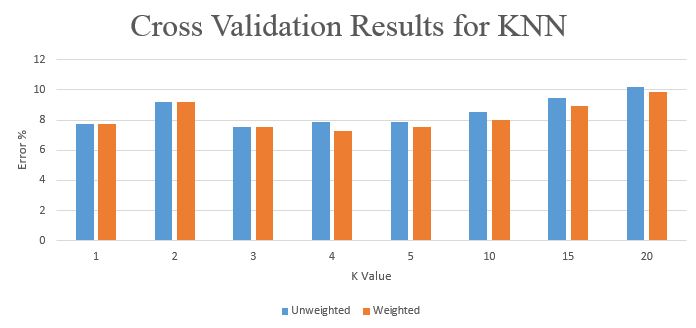
\includegraphics[width=406px]{KNN_CrossValidation.png}
\end{center}

Our cross validation results suggest that running weighted KNN with $K = 4$
yields the most successful classification rate. One caveat to this is that our
cross validation code ran using 5,000 training samples instead of the 42,000
samples in our full training set. It is possible that data we used to cross
validate is no representative of the full data set.

\subsection{Results}

Our KNN implementation was extremely successful, correctly classifying 96.857\%
of the testing samples. One downside to it however is the runtime. Training is
near instantaneous since the algorithm simply loads the data into an array. To
classify a sample the algorithm needs to compute the euclidean distance between
the testing sample and every training sample. In the case of the full data set
this is 42,000 samples, each of which has 768 dimensions. As a result, each
testing sample takes approximately. Altogether it takes close to 8 hours to
classify all 28,000 testing samples.

\section{Kernelized Perceptron}
\subsection{Overview}

The perceptron algorithm attempts to separate a training data set into two
classes and attempts to classify future testing samples as belonging to one of
these two classes. It does this by storing a list of all the mistakes it has
made previously and using this knowledge to adjust future predictions in the
hopes of improving classification accuracy. 

In its most basic implementation, the perceptron algorithm divides the data
linearly. However, the data is often not linearly separable. To address this
issue we use a kernel function to create a non-linear decision boundary. This
allows us to have a more complex decision boundary which potentially fits the
data better.

\subsection{Implementation Details}

Before we can begin classifying test points, we need to train the perceptron
algorithm using our training data set. The training process attempts
to classify each training point sequentially. If the perceptron correctly
classifies the point nothing changes and the training process moves on to the
next training sample. If the training sample is incorrectly classified, however,
the mistake is added to an array of mistakes which is taken into consideration
for future classifications.

One problem that needs to be addressed is that a standard perceptron is a binary
classifier meaning it selects between one of two classes. We resolved this issue
by training $10 \choose 2 = 45$ classifiers. Each classifier is responsible for
classifying between two digits. For example, we would train a perceptron to
classify between 0 and 1, and a second to classify between 0 and 2, and so
on. When we classify we vote between all of our trained classifiers and output
the majority element.

The actual classification is performed by:

\begin{center}
$classify(X) = \sum\limits_{i \in Mistakes}{Y_iK(X_i, X)}$
\end{center}

The kernel function is represented by $K(X_i, X)$. There are a number of choices
for this kernel function.

\subsection{Cross Validation for Kernel Selection}

We implemented two kernel functions to use with our perceptron algorithm. One is
a polynomial kernel which takes the form:

\begin{center}
$Polynomial(x, y, d) = (dot(x, y) + 1)^d$
\end{center}

The second is an exponential kernel:

\begin{center}
$Exponential(x, y, \sigma) = exp(-\frac{||x - y||}{2\sigma^2})$
\end{center}

Both of these kernels have a parameter which needs to be tuned, $d$ in the case of
the polynomial kernel and $\sigma$ in the case of the exponential kernel. We
used cross validation to find out which kernel gave us the best result as well
as which value of $d$ and $\sigma$ was optimal.

\begin{table}[ht]
\textbf{\caption{Perceptron Cross Validation Success Rates}} % title
\centering
\begin{tabular}{c | c c }
Kernel & $d, \sigma = 5$ & $d, \sigma = 10$ \\
\hline
Polynomial & 95.67\% & 94.52\% \\
Exponential & 93.84\% & 96.3\% \\ [1ex]
\end{tabular}
\label{table:perceptron}
\end{table}

\begin{center}
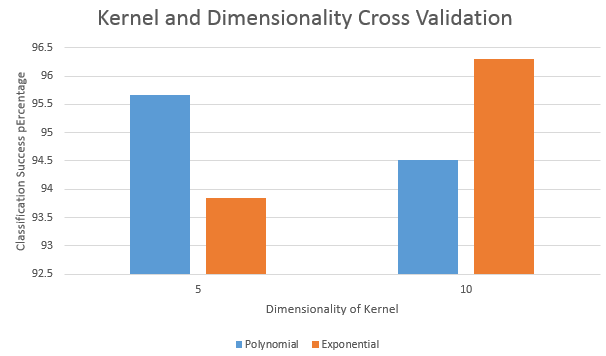
\includegraphics[width=406px]{Perceptron_CrossValidation.png}
\end{center}


\subsection{Results}

Our cross validation indicates that the exponential kernel with a $\sigma$ of 10
leads to the highest success rate of 96.3\%. An interesting observation is that
our polynomial kernel actually became less successful when it's dimension was
increased whereas the exponential kernel got better. We suspect that this is
because the polynomial kernel began to overfit the training data.

Finally, the runtime of the perceptron algorithm is a little over an hour. It
takes approximately 45 minutes to train and about 20 minutes to test the
data. The faster runtime allowed us to cross validate on the full data set.

\section{Conclusion}
Despite its seeming simplicity, we found that KNN was extremely successful
when classifying data points in the Kaggle set.

\begin{center}
\begin{tabular}{ c| c c}
	\hline
Algorithm & Percent Success & runtime\\
	\hline
Nearest Neighbors, $k = 4$   & 96.857\% & $\sim$8 hours\\
Perceptron   & 96.300\%  & $\sim$1 hour\\
\end{tabular}
\end{center}

Table 4 summarizes the accuracy and runtimes of weighted KNN with $K = 4$ and
perceptron with the polynomial kernel and $d = 10$. KNN is clearly more
accurate, however because perceptron is 8x faster and almost as accurate, there
could be many cases where it is a better choice.

In addition to being faster, perceptron likely has a lower memory
footprint. While KNN must store every sample in the training set, perceptron
only stores mistakes which will be a subset of the entire training set.

\section{Future Work}
There are three specific expansions to our work we would have liked to explore
had we had time.

\begin{itemize}
\item Expanded cross validation for KNN using the full training set. This would
  help validate that the weighted voting algorithm with $K = 4$ leads to the
  most accurate. 
\item More kernels and a greater assortment of $\sigma$ and $d$ values to
  see if we can increase the effectiveness of the perceptron algorithm. 
\item An SVM implementation which regularizes the data to avoid overfitting. If
  the perceptron implementation overfits the data, this would be a potential
  way to increase the accuracy.
\end{itemize}


\begingroup
\renewcommand{\section}[2]{}%
%\renewcommand{\chapter}[2]{}% for other classes
\bibliographystyle{unsrt}
\bibliography{references}	
\endgroup




\end{document}

